\subsubsection{Test \ref{test13}, \enquote{Has Cycles} button correctly shows \enquote{The graph has cycles} for a cyclic graph.}
Input:  5 Vertices created, A, B, C, D, and E.  Edge lines exist between (A, B), (A, C), (A, D), (A, E), and (D, E). Click on the \enquote{Has Cycles?} button, observe the message in the status bar.
\newline
\newline
Expected output: The status bar should display \enquote{The graph has cycles.}
\begin{figure}[ht]
    \centering
    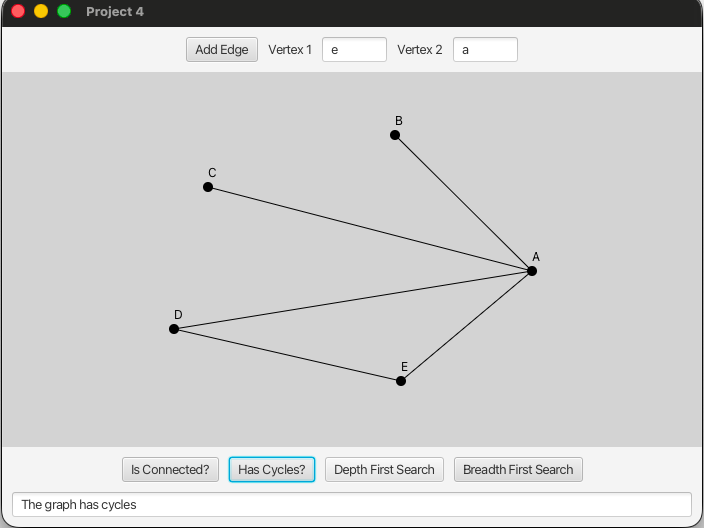
\includegraphics[width=0.65\textwidth]{images/test13.png}
    \caption{test \ref{test13}}
\end{figure}
